\begin{figure}[h!]
    \centering
    \begin{minipage}{0.20\textwidth}
    \centering
    \textbf{Eclipse Dataset}
    
    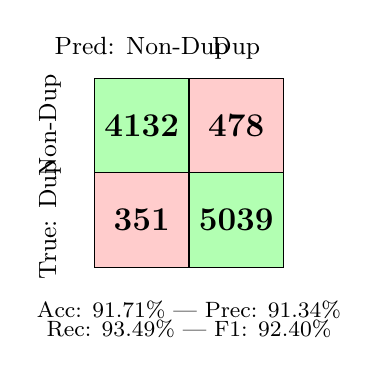
\begin{tikzpicture}[scale=0.6]
      % Matrix cells
      \draw[fill=green!30] (0,2) rectangle (2,4) node[pos=0.5, font=\large\bfseries] {4132};
      \draw[fill=red!20] (2,2) rectangle (4,4) node[pos=0.5, font=\large\bfseries] {478};
      \draw[fill=red!20] (0,0) rectangle (2,2) node[pos=0.5, font=\large\bfseries] {351};
      \draw[fill=green!30] (2,0) rectangle (4,2) node[pos=0.5, font=\large\bfseries] {5039};
      
      % Labels
      \node[above] at (1,4.2) {\small Pred: Non-Dup};
      \node[above] at (3,4.2) {\small Dup};
      \node[rotate=90, anchor=south] at (-0.5,3) {\small Non-Dup};
      \node[rotate=90, anchor=south] at (-0.5,1) {\small True: Dup};
      
      % Metrics
      \node[below, font=\footnotesize] at (2,-0.5) {Acc: 91.71\% | Prec: 91.34\%};
      \node[below, font=\footnotesize] at (2,-0.9) {Rec: 93.49\% | F1: 92.40\%};
    \end{tikzpicture}
    \end{minipage}
    \hfill
    \begin{minipage}{0.20\textwidth}
    \centering
    \textbf{Thunderbird Dataset}
    
    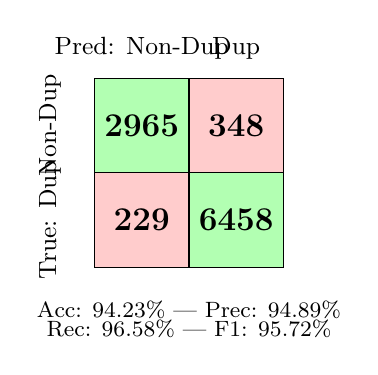
\begin{tikzpicture}[scale=0.6]
      % Matrix cells
      \draw[fill=green!30] (0,2) rectangle (2,4) node[pos=0.5, font=\large\bfseries] {2965};
      \draw[fill=red!20] (2,2) rectangle (4,4) node[pos=0.5, font=\large\bfseries] {348};
      \draw[fill=red!20] (0,0) rectangle (2,2) node[pos=0.5, font=\large\bfseries] {229};
      \draw[fill=green!30] (2,0) rectangle (4,2) node[pos=0.5, font=\large\bfseries] {6458};
      
      % Labels
      \node[above] at (1,4.2) {\small Pred: Non-Dup};
      \node[above] at (3,4.2) {\small Dup};
      \node[rotate=90, anchor=south] at (-0.5,3) {\small Non-Dup};
      \node[rotate=90, anchor=south] at (-0.5,1) {\small True: Dup};
      
      % Metrics
      \node[below, font=\footnotesize] at (2,-0.5) {Acc: 94.23\% | Prec: 94.89\%};
      \node[below, font=\footnotesize] at (2,-0.9) {Rec: 96.58\% | F1: 95.72\%};
    \end{tikzpicture}
    \end{minipage}
    \caption{Confusion matrices visualizing classification results on both datasets. Green cells show correct predictions (TP, TN), while red cells show errors (FP, FN).}
    \label{fig:confusion_matrices}
    \end{figure}